% Definitions: research/METHODS.md, research/METRICS.md; src/sparsity_research/ceilings.py.
% Training settings: Analysis018 tables/training-protocol.md; Runs004/018/019/032/034 configs and manifests.
% Cohorts/evaluation: Analysis024 data/paper-checkpoints.json; Analysis018 figure_data.json.
% Baseline trajectories: Analysis021 observations/O007-a0-optimization.md;
% relabeled without changing data in Analysis024 observations/040-experimental-setup.md.
\section{Experimental setup details}
\label{app:experiment}

\subsection{Pythia architecture and intervention sites}
\label{app:sites}

Table~\ref{tab:sites} specifies the dimensions and positions of the sites in
Figure~\ref{fig:pythia-block}, for one sequence. Here $T$ is sequence length,
$d$ the hidden width, $d_f$ the FFN width, and $H$ the number of attention
heads, each of dimension $d_h=d/H$. The same sites and threshold are used
in every layer of a model.

\begin{table}[ht]
\centering\small
\caption{Activation shapes and intervention positions for one sequence.}
\label{tab:sites}
\vspace{4pt}
\begin{tabularx}{\linewidth}{@{}lllX@{}}
\toprule
Site & Shape & Following matrix product & Position \\
\midrule
$a$ & $T\!\times\!d$ & QKV projection & After attention LayerNorm \\
$m$ & $T\!\times\!d$ & FFN up projection & After FFN LayerNorm \\
$h$ & $T\!\times\!d_f$ & FFN down projection & Activation-function output \\
$q,k$ & $H\!\times\!T\!\times\!d_h$ & Attention scores & After RoPE \\
$v$ & $H\!\times\!T\!\times\!d_h$ & Probability--value & After the QKV split \\
$z$ & $T\!\times\!d$ & Attention-output projection & Concatenated attention context \\
\bottomrule
\end{tabularx}
\end{table}

\FloatBarrier
\subsection{Architecture-specific sparsity ceilings}
\label{app:architecture-counts}

For one sequence, a Pythia block contains $3Td^2$ scalar multiplications
in the QKV projection, $Td^2$ in the attention-output projection,
$Td d_f$ in each FFN projection, and $dT(T+1)/2$ in each of $QK$ and $PV$.
With $L$ layers and vocabulary size $V_{\mathrm{vocab}}$, the per-sequence
counts are
\begin{equation}
\begin{split}
C_{\mathrm{block}}&=T(4d^2+2dd_f)+dT(T+1),\\
C_{\mathrm{model}}&=LC_{\mathrm{block}}+TdV_{\mathrm{vocab}}.
\end{split}
\label{eq:denominator}
\end{equation}
The ceiling can be calculated from these per-sequence counts because
numerator and denominator scale equally with the number of sequences.
Since $d_f=4d$, the counts contributing to the ceiling in each layer are
$0$ for $T_0/P_0$, $4Td^2$ for $T_1/P_0$ and $T_1/P_1$, $12Td^2$ for
all $T_4$ recipes, and $C_{\mathrm{block}}$ for all $T_7$ recipes.
Multiplying by $L$ and dividing by $C_{\mathrm{model}}$ gives $\Smax$;
pressure placement does not change this calculation.

Table~\ref{tab:interventions} uses $V_{\mathrm{vocab}}=50{,}304$ and
$(L,d)=(6,128),(6,512),(24,1{,}024)$ for 14M, 70M and 410M, respectively,
with the common sequence length in Table~\ref{tab:training-settings}.%
\footnote{Pinned architecture configurations:
\href{https://huggingface.co/EleutherAI/pythia-14m-deduped/blob/7386d9a4ae45aef494a6e704910394def3037fc5/config.json}{14M},
\href{https://huggingface.co/EleutherAI/pythia-70m-deduped/blob/e93a9faa9c77e5d09219f6c868bfc7a1bd65593c/config.json}{70M}, and
\href{https://huggingface.co/EleutherAI/pythia-410m-deduped/blob/b5e8535141902c0e985cea61fd02afe7fe86af32/config.json}{410M}.}

\subsection{Training and evaluation}
\label{app:training-protocol}
\label{app:evaluation}

All sizes use the Pythia-14M-deduped tokenizer, initialization and data-order
seeds of 1234, and one training seed per condition. Shared optimizer settings
are AdamW with $\beta=(0.9,0.95)$, $\epsilon=10^{-8}$, weight decay $0.1$,
gradient-norm limit $1$, and zero attention and hidden dropout. Training
lasts 712 optimizer updates, with 1\% linear warmup followed by cosine
learning-rate decay. Table~\ref{tab:training-settings} separates
the size-dependent learning rates and microbatches from the common effective
batch size. The microbatch size is the number of sequences processed together;
gradient accumulation combines several microbatches before one optimizer update.

\begin{table}[htbp]
\centering\small
\caption{\textbf{Training settings across model sizes.}
Effective batch size equals microbatch size times gradient accumulation.
The common training budget gives fewer tokens per parameter at larger sizes.}
\label{tab:training-settings}
\begin{tabular}{@{}lrrr@{}}
\toprule
Setting & 14M & 70M & 410M \\
\midrule
Parameters & 14,067,712 & 70,426,624 & 405,334,016 \\
Peak learning rate & $10^{-3}$ & $10^{-3}$ & $3\!\times\!10^{-4}$ \\
Minimum learning rate & $10^{-4}$ & $10^{-4}$ & $3\!\times\!10^{-5}$ \\
Microbatch (sequences) & 32 & 4 & 4 \\
Gradient accumulation (microbatches) & 32 & 256 & 256 \\
Effective batch (sequences/update) & 1,024 & 1,024 & 1,024 \\
Sequence length & 2,048 & 2,048 & 2,048 \\
Tokens per parameter & 106.14 & 21.20 & 3.68 \\
\bottomrule
\end{tabular}
\end{table}
\FloatBarrier

The 14M study includes $T_0/P_0$, $T_1/P_0$, $T_1/P_1$ with either L1 or
OL1, and the $T_4$ and $T_7$ recipes with $P_0$, $P_h$ or $P_{\mathrm{all}}$.
The 70M study includes both controls and the $T_4$ and $T_7$ recipes with $P_h$
or $P_{\mathrm{all}}$; at 410M, only the controls and $P_{\mathrm{all}}$
recipes are run. All sweeps use the grids in Table~\ref{tab:interventions}.
We evaluate final checkpoints without validation-based checkpoint selection.
The main figures report validation loss and model-wide sparsity over the
same validation sequences, as defined in Appendix~\ref{app:accounting}.

Figure~\ref{fig:a0-optimization} provides training context for the cross-size
loss comparison. These trajectories do not establish convergence, and the
410M learning-rate range differs from that of the smaller models.

\begin{figure}[htbp]
\centering
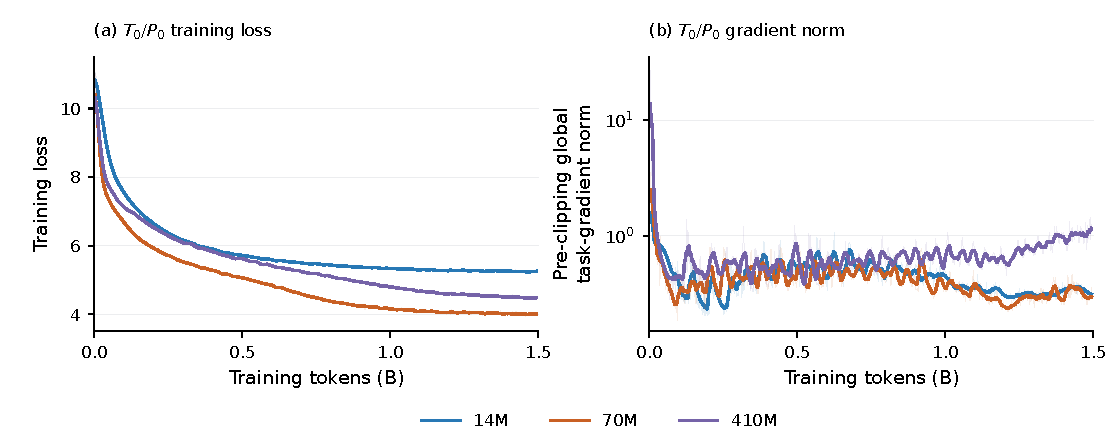
\includegraphics[width=\linewidth]{figures/19-base-model-optimization.pdf}
\caption{\textbf{Base-model ($T_0/P_0$) training across model sizes.}
\textbf{(a)} Training loss and \textbf{(b)} gradient norm before clipping
(logarithmic scale). Faint lines show individual updates; solid lines show
centered nine-update means, with shorter windows at the ends. Gradient norms
are computed after accumulation and are not normalized by parameter count.}
\label{fig:a0-optimization}
\end{figure}

\FloatBarrier
% Source observation: analyses/018-2026-09-08-results-materials/observations/O012-manuscript-results.md
% Evidence: Analysis 018 O001--O004/O007/O011, figure_data.json and tables/training-protocol.md.
% Complete clipping: Run 030 observations/O001--O003 and results/*.
% Signed distributions: Run 031 results/histograms/*.json.gz.
% Composite density/accounting figure: Analysis 021 observations/O005-distributions-and-operations.md; 04_distributions_and_operations.py.
% Kernel contract: Run 029 observations/06-implementation-and-claim-audit.md.
% Kernel compatibility/predicate revision: Analysis 018 O015; Run 022 README, Run 025 SOURCE_AUDIT.md.
% Kernel adoption: Analysis 021 observations/O009-kernel-realization-v2.md;
% investigation/observations/O001-kernel-investigation.md and 01_extract.py--03_plot.py.
% Per-checkpoint latency table: Analysis 021 / 08_kernel_manuscript_table.py.
% Generated tables: Analysis 018 / 03_manuscript_tables.py.
% Figure 1 two-size extension: analyses/024-2026-09-17-h-only-kernel-latency/observations/025-matched-quality-latency.md;
% generating analysis: analyses/024-2026-09-17-h-only-kernel-latency/16_plot_matched_quality_latency.py.
% A0 histories: analyses/021-2026-09-10-training-results-figures/06_a0_optimization.py;
% observations/O007-a0-optimization.md; data/a0-optimization.json.
\section{Complete results and supporting diagnostics}
\label{app:complete-results}

The following tables report the original 64 trained endpoints and the ten
additional 70M h-only endpoints, the 29 original paired
14M contrasts, 25 additional pressure-scope contrasts, and all 15 cross-scale
broad-pressure recipe comparisons. They retain
dominated settings as well as favorable ones. Each entry summarizes one
trained model on complete validation. Sparsity percentages are formed from pooled integer
product counts. The endpoint table uses the common seven-site sparsity-ceiling
denominator from Table~\ref{tab:interventions}, rather than a different denominator
for each recipe. Here $U_{\mathrm{arch}}=\Smodel/\Smax(\mathrm{A7})$ denotes
this common-reference ratio, retained for the complete endpoint table.

% Source: Analysis 021 pressure-scope/tables.py; 54 original + 10 verified h-only endpoints.
{\small\renewcommand{\arraystretch}{0.95}
\begin{longtable}{@{}lllrrr@{}}
\caption{The original 64 trained endpoints; Table~\ref{tab:70m-h-only-endpoints} adds the ten 70M h-only conditions. $T_i/P_j$ specifies threshold and pressure scope; $P_0$ means no pressure. $U_{\mathrm{arch}}$ uses the common seven-site ceiling within each size. H-only losses use ordinary final validation; other losses use the logical diagnostic pass (Appendix~\ref{app:evaluation}). Rounded zero sparsity need not be exactly zero.}\label{tab:trained-endpoints}\\
\toprule
Size & Recipe & Parameter & Loss & $\Smodel$ (\%) & $U_{\mathrm{arch}}$ (\%) \\
\midrule
\endfirsthead
\multicolumn{6}{l}{\tablename~\thetable{} (continued)}\\
\toprule
Size & Recipe & Parameter & Loss & $\Smodel$ (\%) & $U_{\mathrm{arch}}$ (\%) \\
\midrule
\endhead
\bottomrule\endfoot
14M & A0 & --- & 5.2086 & 0.000 & 0.000 \\
14M & A1-H & --- & 5.2696 & 2.714 & 9.061 \\
14M & A1-H-L1 & $\lambda=0.05$ & 5.2061 & 3.142 & 10.489 \\
14M & A1-H-L1 & $\lambda=0.1$ & 5.1655 & 3.336 & 11.139 \\
14M & A1-H-L1 & $\lambda=0.5$ & 5.1127 & 3.788 & 12.645 \\
14M & A1-H-L1 & $\lambda=1$ & 5.1023 & 3.949 & 13.185 \\
14M & A1-H-OL1 & $\lambda=0.05$ & 5.1981 & 3.145 & 10.501 \\
14M & A1-H-OL1 & $\lambda=0.1$ & 5.1594 & 3.339 & 11.146 \\
14M & A1-H-OL1 & $\lambda=0.5$ & 5.1102 & 3.768 & 12.580 \\
14M & A1-H-OL1 & $\lambda=1$ & 5.1212 & 3.938 & 13.149 \\
14M & $T_4/P_0$ & $\kappa=0$ & 5.4705 & 7.212 & 24.078 \\
14M & $T_4/P_0$ & $\kappa=0.01$ & 5.4665 & 7.414 & 24.752 \\
14M & $T_4/P_0$ & $\kappa=0.05$ & 5.4341 & 8.206 & 27.396 \\
14M & $T_4/P_0$ & $\kappa=0.1$ & 5.4197 & 8.953 & 29.891 \\
14M & $T_4/P_0$ & $\kappa=0.5$ & 5.6597 & 10.216 & 34.106 \\
14M & $T_4/P_h$ & $\kappa=0$ & 5.2157 & 8.409 & 28.076 \\
14M & $T_4/P_h$ & $\kappa=0.01$ & 5.2045 & 8.586 & 28.665 \\
14M & $T_4/P_h$ & $\kappa=0.05$ & 5.1956 & 9.036 & 30.167 \\
14M & $T_4/P_h$ & $\kappa=0.1$ & 5.2287 & 9.343 & 31.194 \\
14M & $T_4/P_h$ & $\kappa=0.5$ & 5.7227 & 10.227 & 34.146 \\
14M & $T_4/P_4$ & $\kappa=0$ & 5.4583 & 7.810 & 26.075 \\
14M & $T_4/P_4$ & $\kappa=0.01$ & 5.4583 & 8.587 & 28.668 \\
14M & $T_4/P_4$ & $\kappa=0.05$ & 5.4898 & 10.456 & 34.910 \\
14M & $T_4/P_4$ & $\kappa=0.1$ & 5.5483 & 11.394 & 38.041 \\
14M & $T_4/P_4$ & $\kappa=0.5$ & 6.0380 & 12.713 & 42.446 \\
14M & $T_7/P_0$ & $\kappa=0$ & 5.4684 & 7.218 & 24.097 \\
14M & $T_7/P_0$ & $\kappa=0.01$ & 5.4588 & 7.618 & 25.433 \\
14M & $T_7/P_0$ & $\kappa=0.05$ & 5.4379 & 9.127 & 30.471 \\
14M & $T_7/P_0$ & $\kappa=0.1$ & 5.4287 & 10.425 & 34.805 \\
14M & $T_7/P_0$ & $\kappa=0.5$ & 5.7029 & 15.387 & 51.371 \\
14M & $T_7/P_h$ & $\kappa=0$ & 5.2198 & 8.399 & 28.042 \\
14M & $T_7/P_h$ & $\kappa=0.01$ & 5.1981 & 8.856 & 29.567 \\
14M & $T_7/P_h$ & $\kappa=0.05$ & 5.1950 & 10.126 & 33.807 \\
14M & $T_7/P_h$ & $\kappa=0.1$ & 5.2374 & 10.904 & 36.403 \\
14M & $T_7/P_h$ & $\kappa=0.5$ & 5.7320 & 16.664 & 55.634 \\
14M & $T_7/P_7$ & $\kappa=0$ & 5.4802 & 7.054 & 23.551 \\
14M & $T_7/P_7$ & $\kappa=0.01$ & 5.4758 & 7.723 & 25.786 \\
14M & $T_7/P_7$ & $\kappa=0.05$ & 5.4628 & 9.863 & 32.929 \\
14M & $T_7/P_7$ & $\kappa=0.1$ & 5.4295 & 11.797 & 39.385 \\
14M & $T_7/P_7$ & $\kappa=0.5$ & 5.8294 & 27.483 & 91.755 \\
70M & A0 & --- & 4.0998 & 0.000 & 0.001 \\
70M & A1-H & --- & 4.2227 & 10.066 & 20.366 \\
70M & $T_4/P_4$ & $\kappa=0$ & 4.8054 & 25.673 & 51.944 \\
70M & $T_4/P_4$ & $\kappa=0.01$ & 4.8229 & 26.224 & 53.060 \\
70M & $T_4/P_4$ & $\kappa=0.05$ & 4.8742 & 28.490 & 57.644 \\
70M & $T_4/P_4$ & $\kappa=0.1$ & 4.9439 & 30.574 & 61.861 \\
70M & $T_4/P_4$ & $\kappa=0.5$ & 5.3895 & 35.596 & 72.022 \\
70M & $T_7/P_7$ & $\kappa=0$ & 4.9412 & 23.562 & 47.674 \\
70M & $T_7/P_7$ & $\kappa=0.01$ & 4.9364 & 24.226 & 49.017 \\
70M & $T_7/P_7$ & $\kappa=0.05$ & 4.9637 & 26.524 & 53.666 \\
70M & $T_7/P_7$ & $\kappa=0.1$ & 4.9501 & 28.694 & 58.056 \\
70M & $T_7/P_7$ & $\kappa=0.5$ & 5.2159 & 40.602 & 82.150 \\
410M & A0 & --- & 4.5475 & 0.011 & 0.013 \\
410M & A1-H & --- & 4.6513 & 21.050 & 24.127 \\
410M & $T_4/P_4$ & $\kappa=0$ & 5.6921 & 38.339 & 43.944 \\
410M & $T_4/P_4$ & $\kappa=0.01$ & 5.6914 & 39.149 & 44.873 \\
410M & $T_4/P_4$ & $\kappa=0.05$ & 5.6789 & 42.125 & 48.283 \\
410M & $T_4/P_4$ & $\kappa=0.1$ & 5.6789 & 45.688 & 52.367 \\
410M & $T_4/P_4$ & $\kappa=0.5$ & 5.1910 & 71.591 & 82.058 \\
410M & $T_7/P_7$ & $\kappa=0$ & 5.4263 & 41.121 & 47.133 \\
410M & $T_7/P_7$ & $\kappa=0.01$ & 5.4331 & 41.478 & 47.542 \\
410M & $T_7/P_7$ & $\kappa=0.05$ & 5.4679 & 44.053 & 50.494 \\
410M & $T_7/P_7$ & $\kappa=0.1$ & 5.4907 & 48.998 & 56.161 \\
410M & $T_7/P_7$ & $\kappa=0.5$ & 5.1207 & 80.616 & 92.401 \\
\end{longtable}}

% Source: analyses/024-2026-09-17-h-only-kernel-latency/data/14m-70m-quality-sparsity-latency.json
% Observation: analyses/024-2026-09-17-h-only-kernel-latency/observations/025-matched-quality-latency.md
% Generating analysis: 16_plot_matched_quality_latency.py; rounded directly from trained_points.
\begin{table}[!htbp]
\centering\small
\caption{Additional 70M h-only endpoints in Figure~\ref{fig:quality-sparsity-overview}. Loss uses ordinary reloaded final validation; sparsity uses canonical FP16 logical counts. $U_{\mathrm{arch}}$ uses the common seven-site ceiling, as in Table~\ref{tab:trained-endpoints}. Together the two tables cover all 74 trained conditions.}
\label{tab:70m-h-only-endpoints}
\begin{tabular}{@{}llrrr@{}}
\toprule
Recipe & $\kappa$ & Loss & $\Smodel$ (\%) & $U_{\mathrm{arch}}$ (\%) \\
\midrule
$T_4/P_h$ & 0 & 4.6065 & 25.792 & 52.185 \\
$T_4/P_h$ & 0.01 & 4.6185 & 25.971 & 52.547 \\
$T_4/P_h$ & 0.05 & 4.5964 & 26.566 & 53.752 \\
$T_4/P_h$ & 0.1 & 4.7020 & 27.218 & 55.071 \\
$T_4/P_h$ & 0.5 & 5.3057 & 29.236 & 59.153 \\
$T_7/P_h$ & 0 & 4.6508 & 25.786 & 52.173 \\
$T_7/P_h$ & 0.01 & 4.6122 & 26.009 & 52.624 \\
$T_7/P_h$ & 0.05 & 4.6670 & 26.895 & 54.416 \\
$T_7/P_h$ & 0.1 & 4.7189 & 27.779 & 56.206 \\
$T_7/P_h$ & 0.5 & 5.3372 & 32.233 & 65.216 \\
\bottomrule
\end{tabular}
\end{table}

% Editorial labels: OL1(all) makes the historical broad-pressure scope explicit; numerical rows unchanged.
% Generated by Analysis 018 / 03_manuscript_tables.py.
\begin{table}[p]\centering\small\renewcommand{\arraystretch}{0.95}
\caption{All 29 Pythia-14M contrasts, treatment minus reference. When both recipes have a swept parameter, its value is matched; A0 and A1-H are fixed controls.}\label{tab:paired-effects-full}
\begin{tabular}{@{}llrr@{}}
\toprule
Treatment $-$ reference & Parameter & $\Delta$ loss & $\Delta\Smodel$ (pp) \\
\midrule
A1-H $-$ A0 & --- & +0.0611 & +2.714 \\
A1-H-L1 $-$ A1-H & $\lambda=0.05$ & -0.0635 & +0.427 \\
A1-H-L1 $-$ A1-H & $\lambda=0.1$ & -0.1042 & +0.622 \\
A1-H-L1 $-$ A1-H & $\lambda=0.5$ & -0.1569 & +1.073 \\
A1-H-L1 $-$ A1-H & $\lambda=1$ & -0.1674 & +1.235 \\
A1-H-OL1 $-$ A1-H-L1 & $\lambda=0.05$ & -0.0081 & +0.004 \\
A1-H-OL1 $-$ A1-H-L1 & $\lambda=0.1$ & -0.0061 & +0.002 \\
A1-H-OL1 $-$ A1-H-L1 & $\lambda=0.5$ & -0.0025 & -0.020 \\
A1-H-OL1 $-$ A1-H-L1 & $\lambda=1$ & +0.0189 & -0.011 \\
A4 $-$ A1-H & $\kappa=0$ & +0.2009 & +4.498 \\
A4 $-$ A1-H & $\kappa=0.01$ & +0.1969 & +4.700 \\
A4 $-$ A1-H & $\kappa=0.05$ & +0.1645 & +5.492 \\
A4 $-$ A1-H & $\kappa=0.1$ & +0.1500 & +6.239 \\
A4 $-$ A1-H & $\kappa=0.5$ & +0.3900 & +7.501 \\
A4-OL1(all) $-$ A4 & $\kappa=0$ & -0.0122 & +0.598 \\
A4-OL1(all) $-$ A4 & $\kappa=0.01$ & -0.0082 & +1.173 \\
A4-OL1(all) $-$ A4 & $\kappa=0.05$ & +0.0556 & +2.251 \\
A4-OL1(all) $-$ A4 & $\kappa=0.1$ & +0.1286 & +2.441 \\
A4-OL1(all) $-$ A4 & $\kappa=0.5$ & +0.3783 & +2.498 \\
A7 $-$ A4 & $\kappa=0$ & -0.0021 & +0.006 \\
A7 $-$ A4 & $\kappa=0.01$ & -0.0077 & +0.204 \\
A7 $-$ A4 & $\kappa=0.05$ & +0.0038 & +0.921 \\
A7 $-$ A4 & $\kappa=0.1$ & +0.0090 & +1.472 \\
A7 $-$ A4 & $\kappa=0.5$ & +0.0432 & +5.171 \\
A7-OL1(all) $-$ A7 & $\kappa=0$ & +0.0118 & -0.163 \\
A7-OL1(all) $-$ A7 & $\kappa=0.01$ & +0.0170 & +0.106 \\
A7-OL1(all) $-$ A7 & $\kappa=0.05$ & +0.0249 & +0.736 \\
A7-OL1(all) $-$ A7 & $\kappa=0.1$ & +0.0008 & +1.372 \\
A7-OL1(all) $-$ A7 & $\kappa=0.5$ & +0.1265 & +12.096 \\
\bottomrule
\end{tabular}
\end{table}

% Source: Analysis 021 pressure-scope/tables.py; matched reported losses.
\begin{table}[p]\centering\small
\caption{Pressure-scope increments and threshold-placement contrasts at 14M. Each row subtracts the reference at the same $\kappa$. These are single-seed comparisons.}\label{tab:pressure-scope-full}
\begin{tabular}{@{}llrr@{}}
\toprule
Treatment $-$ reference & $\kappa$ & $\Delta L$ & $\Delta\Smodel$ (pp) \\
\midrule
$T_4/P_h$ $-$ $T_4/P_0$ & 0 & -0.2548 & +1.197 \\
$T_4/P_h$ $-$ $T_4/P_0$ & 0.01 & -0.2620 & +1.172 \\
$T_4/P_h$ $-$ $T_4/P_0$ & 0.05 & -0.2385 & +0.830 \\
$T_4/P_h$ $-$ $T_4/P_0$ & 0.1 & -0.1910 & +0.390 \\
$T_4/P_h$ $-$ $T_4/P_0$ & 0.5 & +0.0630 & +0.012 \\
$T_4/P_4$ $-$ $T_4/P_h$ & 0 & +0.2425 & -0.599 \\
$T_4/P_4$ $-$ $T_4/P_h$ & 0.01 & +0.2538 & +0.001 \\
$T_4/P_4$ $-$ $T_4/P_h$ & 0.05 & +0.2942 & +1.421 \\
$T_4/P_4$ $-$ $T_4/P_h$ & 0.1 & +0.3196 & +2.051 \\
$T_4/P_4$ $-$ $T_4/P_h$ & 0.5 & +0.3153 & +2.486 \\
$T_7/P_h$ $-$ $T_7/P_0$ & 0 & -0.2486 & +1.182 \\
$T_7/P_h$ $-$ $T_7/P_0$ & 0.01 & -0.2607 & +1.238 \\
$T_7/P_h$ $-$ $T_7/P_0$ & 0.05 & -0.2429 & +0.999 \\
$T_7/P_h$ $-$ $T_7/P_0$ & 0.1 & -0.1913 & +0.479 \\
$T_7/P_h$ $-$ $T_7/P_0$ & 0.5 & +0.0292 & +1.277 \\
$T_7/P_7$ $-$ $T_7/P_h$ & 0 & +0.2604 & -1.345 \\
$T_7/P_7$ $-$ $T_7/P_h$ & 0.01 & +0.2777 & -1.133 \\
$T_7/P_7$ $-$ $T_7/P_h$ & 0.05 & +0.2678 & -0.263 \\
$T_7/P_7$ $-$ $T_7/P_h$ & 0.1 & +0.1921 & +0.893 \\
$T_7/P_7$ $-$ $T_7/P_h$ & 0.5 & +0.0974 & +10.819 \\
$T_7/P_h$ $-$ $T_4/P_h$ & 0 & +0.0041 & -0.010 \\
$T_7/P_h$ $-$ $T_4/P_h$ & 0.01 & -0.0064 & +0.270 \\
$T_7/P_h$ $-$ $T_4/P_h$ & 0.05 & -0.0006 & +1.090 \\
$T_7/P_h$ $-$ $T_4/P_h$ & 0.1 & +0.0087 & +1.560 \\
$T_7/P_h$ $-$ $T_4/P_h$ & 0.5 & +0.0094 & +6.436 \\
\bottomrule
\end{tabular}
\end{table}

% Editorial labels: OL1(all) makes the historical broad-pressure scope explicit; numerical rows unchanged.
% Generated by Analysis 018 / 03_manuscript_tables.py.
\begin{table}[p]\centering\small\renewcommand{\arraystretch}{0.95}
\caption{All matched A7-OL1(all) minus A4-OL1(all) comparisons. Negative loss changes and positive sparsity changes favor A7-OL1(all).}\label{tab:scale-pairs-full}
\begin{tabular}{@{}lrrr@{}}
\toprule
Size & $\kappa$ & $\Delta$ loss & $\Delta\Smodel$ (pp) \\
\midrule
14M & 0 & +0.0219 & -0.756 \\
14M & 0.01 & +0.0175 & -0.863 \\
14M & 0.05 & -0.0270 & -0.593 \\
14M & 0.1 & -0.1188 & +0.402 \\
14M & 0.5 & -0.2086 & +14.769 \\
70M & 0 & +0.1358 & -2.110 \\
70M & 0.01 & +0.1135 & -1.998 \\
70M & 0.05 & +0.0895 & -1.966 \\
70M & 0.1 & +0.0062 & -1.880 \\
70M & 0.5 & -0.1736 & +5.006 \\
410M & 0 & -0.2658 & +2.783 \\
410M & 0.01 & -0.2582 & +2.329 \\
410M & 0.05 & -0.2111 & +1.929 \\
410M & 0.1 & -0.1881 & +3.310 \\
410M & 0.5 & -0.0703 & +9.024 \\
\bottomrule
\end{tabular}
\end{table}


\subsection{Activation sparsity and signed-density coverage}
\label{app:density-results}

The seven frozen-checkpoint evaluations in
Figure~\ref{fig:activation-density-full} record signed values after the trained
nonlinearities, with Q/K measured after RoPE. Each checkpoint contributes
2,658,140,160 FFN elements and 1,594,884,096 attention elements across the
complete validation set. Summing integer counts gives the 80:20 weighting
of $h:m$ and equal weighting of $q:k:v$. These pooled distributions are
element-weighted mixtures, not distributions of layer means.

Exact zeros are stored separately from the nonzero histogram. The native
grid spans $[-8,8]$ with 16,000 bins of nominal width 0.001; the figure
combines ten bins at a time and divides by the actual floating-point bin
width and the count of all captured elements. Consequently, a curve's full
integral is the recorded nonzero mass inside that grid, not one. Table~\ref{tab:density-mass}
reports the zero mass and the fractions outside the displayed and native
ranges. Underflow and overflow counts are retained rather than folded into
edge bins. The displayed limits are $[-2.5,3]$ for FFN and $[-4,4]$ for
attention in Figure~\ref{fig:activation-density-full}. The largest omitted
display tail is $6.6719\%$; the native-grid tail is at most $0.7607\%$.
These historical densities cover no h-only multisite checkpoints.
Figures~\ref{fig:moderate-structure} and~\ref{fig:pressure-layer-zeros}
use retained final-validation site counters for all six threshold/pressure
combinations, separating $m$ and $h$. These counts were measured independently
of the signed histogram reruns; small pass-to-pass rounding differences remain
visible. The retained logical-product counters separately decompose model-wide
sparsity into operation contributions at $\kappa=0.05$ and $0.5$.

The diagnostic reruns use FP32 parameters with FP16 autocast and no
additional thresholding. Their maximum absolute validation-loss difference
from the retained reference is $6.89\times10^{-5}$, below the specified
$5\times10^{-4}$ tolerance; all 108 threshold-consistency checks pass. Small
rounding differences in exact-zero counts between evaluation passes do not
change the displayed conclusions. Complete per-site and pooled histograms,
counts and checkpoint hashes accompany the data release.

% Source: Analysis 021 pressure-scope/observations/O016-pressure-placement.md.
\begin{figure}[tbp]
\centering
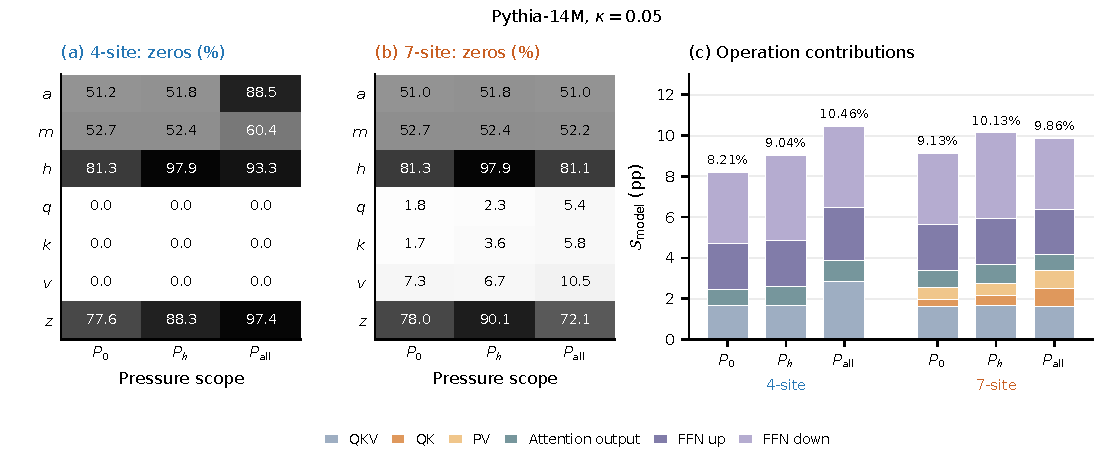
\includegraphics[width=\linewidth]{figures/pressure-scope/appendix-moderate-structure.pdf}
\caption{\textbf{Pressure-scope effects at the moderate threshold $\kappa=0.05$.}
The six 14M recipes use pooled counts and the full-model operation denominator
defined in Appendix~\ref{app:accounting}. H-only pressure concentrates zeros at
$h$ while preserving a different pattern at $m$ and Q/K/V from broad pressure.
Rounded percentages do not establish all-zero or fully dense tensors.}
\label{fig:moderate-structure}
\end{figure}

\begin{figure}[p]
\centering
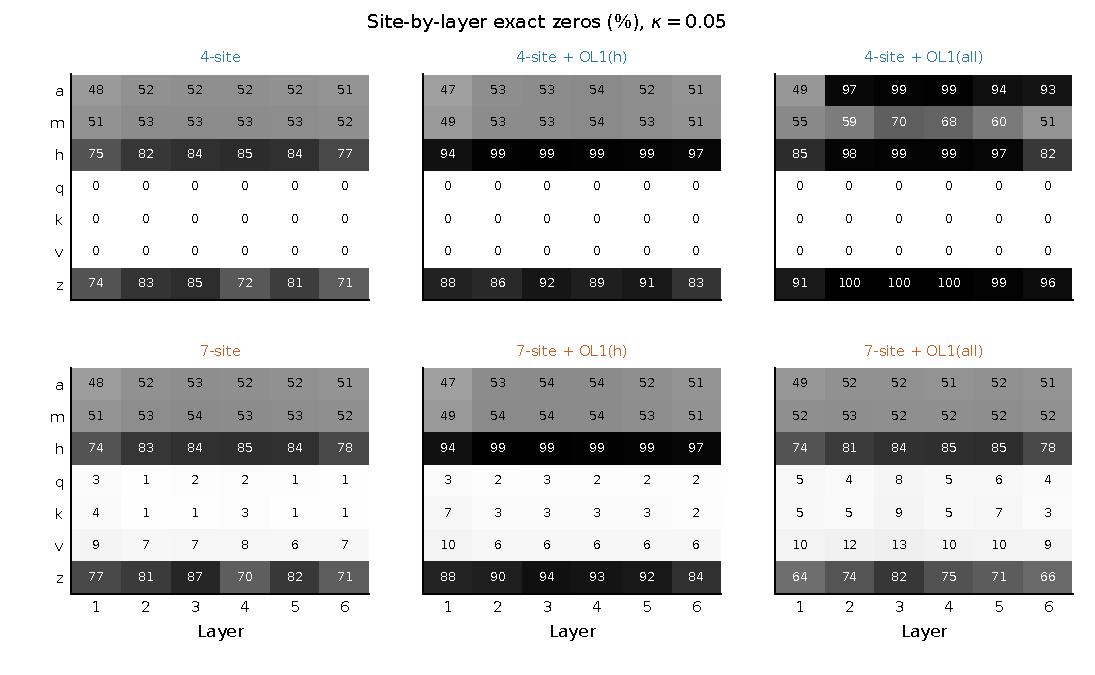
\includegraphics[width=\linewidth,page=1]{figures/pressure-scope/appendix-layer-zeros.pdf}
\includegraphics[width=\linewidth,page=2]{figures/pressure-scope/appendix-layer-zeros.pdf}
\caption{\textbf{Site-by-layer zero fractions under matched pressure scopes.}
The six recipes at $\kappa=0.05$ (top) and $0.5$ (bottom). Each cell pools
integer counts over all 338 validation blocks at one site and layer.
Q/K are post-RoPE; values are rounded to whole percentages, so a displayed
100 does not imply an all-zero tensor. The complete five-threshold counters
and source identities accompany the supplementary data.}
\label{fig:pressure-layer-zeros}
\end{figure}

% Full threshold grid moved from the main text; original Analysis 018 PDF unchanged.
\begin{figure}[tbp]
\centering
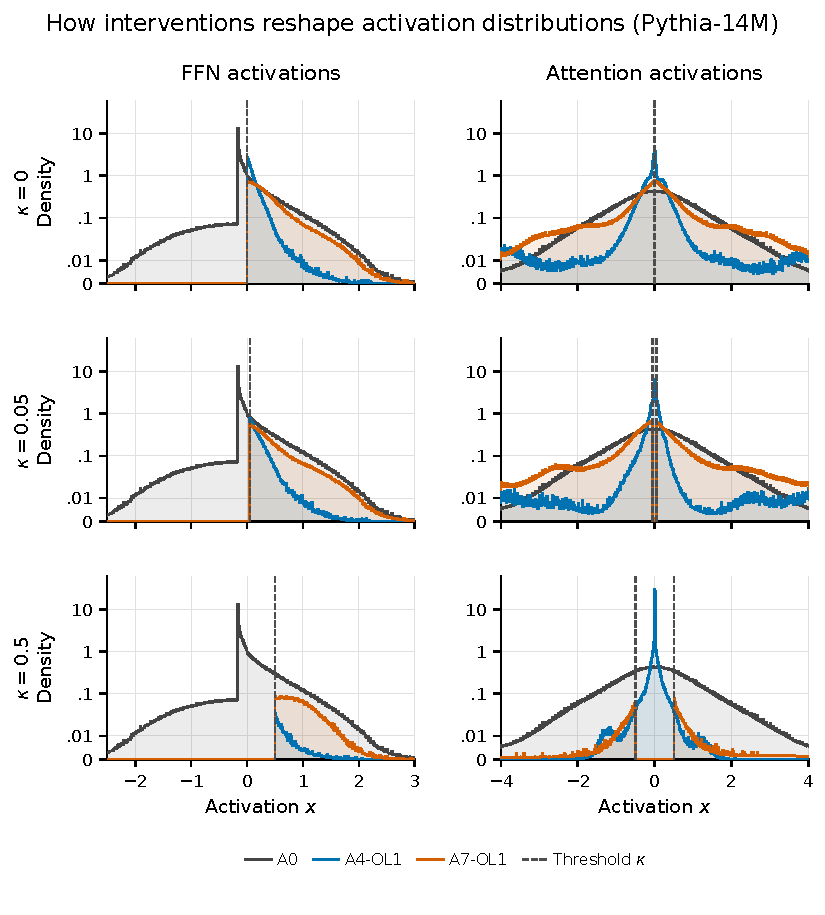
\includegraphics[width=\linewidth]{figures/05-v3-activation-density-grid.pdf}
\caption{\textbf{Interventions reshape FFN and attention distributions differently.}
\textbf{Exact zeros are omitted from the curves and reported in
Table~\ref{tab:density-mass}.} Columns pool FFN $(h,m)$ and attention
$(q,k,v)$ activations; rows use trained thresholds $\kappa=0,0.05,0.5$.
A0 is repeated across rows. Counts are pooled across all layers and validation
blocks, weighting $h:m$ by 80:20 and $q:k:v$ equally. Density divides nonzero
bin counts by all captured elements and bin width, without renormalizing
the visible range. The vertical scale is symlog, linear below 0.01; filled
areas on this scale do not represent probability mass. Dashed lines mark
$+\kappa$ for A4/A7 FFN thresholds and $\pm\kappa$ for A7 attention thresholds.
Q/K are measured after RoPE. A4 leaves $q,k,v$ without direct thresholding or pressure;
A7 targets them directly. The seven checkpoints use no additional post-hoc thresholding.}
\label{fig:activation-density-full}
\end{figure}

\begin{table}[htbp]
\centering\small
\caption{Activation sparsity (the probability mass at zero) omitted from the
density curves, and mass outside their
displayed range (view tail) and the native $[-8,8]$ histogram (grid tail).
Grid tails are a subset of view tails, not an additional mass to add.
All percentages divide integer counts by all captured elements. A0 is
listed once although it is repeated in each figure row. These 14 groups
come from seven checkpoints.}
\label{tab:density-mass}
% Editorial labels: OL1(all) makes the historical broad-pressure scope explicit; numerical rows unchanged.
% Generated by Analysis 018 / 03_manuscript_tables.py.
\begin{tabular}{@{}lllrrr@{}}
\toprule
Recipe & $\kappa$ & Group & Sparsity (\%) & View tail (\%) & Grid tail (\%) \\
\midrule
A0 & --- & FFN & $<0.01$ & 0.1113 & 0.0000 \\
A0 & --- & Attention & $<0.01$ & 2.3929 & 0.4632 \\
A4-OL1(all) & 0 & FFN & 67.22 & 0.0003 & 0.0000 \\
A4-OL1(all) & 0 & Attention & $<0.01$ & 5.1717 & 0.6162 \\
A4-OL1(all) & 0.05 & FFN & 86.71 & 0.0003 & 0.0000 \\
A4-OL1(all) & 0.05 & Attention & $<0.01$ & 5.6601 & 0.7607 \\
A4-OL1(all) & 0.5 & FFN & 99.31 & 0.0001 & 0.0000 \\
A4-OL1(all) & 0.5 & Attention & 0.22 & 0.0003 & 0.0000 \\
A7-OL1(all) & 0 & FFN & 64.52 & 0.0063 & 0.0000 \\
A7-OL1(all) & 0 & Attention & $<0.01$ & 5.4657 & 0.4648 \\
A7-OL1(all) & 0.05 & FFN & 75.29 & 0.0106 & 0.0000 \\
A7-OL1(all) & 0.05 & Attention & 7.26 & 6.6719 & 0.6932 \\
A7-OL1(all) & 0.5 & FFN & 93.64 & 0.0037 & 0.0000 \\
A7-OL1(all) & 0.5 & Attention & 95.60 & 0.2396 & 0.0009 \\
\bottomrule
\end{tabular}

\end{table}

\FloatBarrier
\subsection{Operation contributions to model-wide sparsity}
\label{app:operation-results}

An operation's contribution to $\Smodel$ is its zero-product count divided
by the full model product count. Summing these contributions recovers the
model-wide fraction; summing local activation percentages would not.
Table~\ref{tab:operation-contributions} gives this decomposition at
$\kappa=0.5$. At 14M, extending from A4-OL1(all) to A7-OL1(all) adds attention
opportunity while reducing the contribution from some projections.
At larger sizes, projection work carries more weight in the workload, so
an equal change in activation sparsity need not yield an equal change in
model-wide sparsity. Figure~\ref{fig:operation-accounting} displays the
operation-level view at the same threshold and all three sizes.

\begin{table}[htbp]
\centering\small\setlength{\tabcolsep}{4pt}
\caption{Contributions to $100\Smodel$ in percentage points at
$\kappa=0.5$. All six operations share the same model denominator within
each size. The dense LM head contributes to that denominator but receives
no zero credit. Differences in rounded entries can affect the displayed sum.}
\label{tab:operation-contributions}
% Editorial labels: OL1(all) makes the historical broad-pressure scope explicit; numerical rows unchanged.
% Generated by Analysis 018 / 03_manuscript_tables.py.
\begin{tabular}{@{}lrrrrrr@{}}
\toprule
& \multicolumn{2}{c}{14M} & \multicolumn{2}{c}{70M} & \multicolumn{2}{c}{410M} \\ Operation & A4-OL1(all) & A7-OL1(all) & A4-OL1(all) & A7-OL1(all) & A4-OL1(all) & A7-OL1(all) \\
\midrule
QKV & 3.173 & 2.430 & 8.820 & 6.231 & 17.563 & 16.992 \\
$QK$ & 0.000 & 8.324 & 0.000 & 5.052 & 0.000 & 5.206 \\
$PV$ & 0.057 & 8.449 & 0.011 & 5.371 & 0.008 & 5.858 \\
Attention output & 1.069 & 1.069 & 3.087 & 3.084 & 6.186 & 6.187 \\
FFN up & 4.139 & 2.939 & 11.329 & 8.526 & 22.938 & 21.503 \\
FFN down & 4.275 & 4.272 & 12.350 & 12.338 & 24.895 & 24.869 \\
Total & 12.713 & 27.483 & 35.596 & 40.602 & 71.591 & 80.616 \\
\bottomrule
\end{tabular}

\end{table}

\begin{figure}[htbp]
\centering
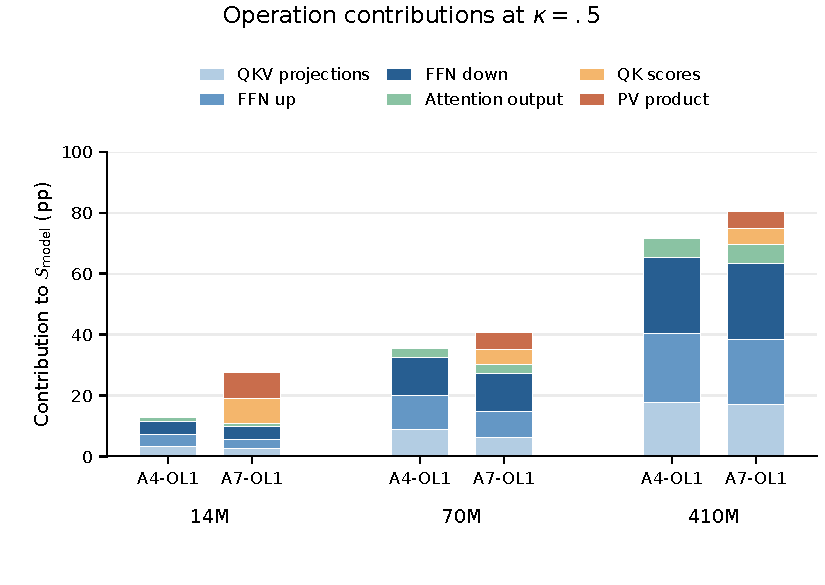
\includegraphics[width=\linewidth]{figures/appendix/04-operation-accounting.pdf}
\caption{Operation accounting for A4-OL1(all) and A7-OL1(all) at $\kappa=0.5$ across
14M, 70M and 410M. Zero-operand
products are counted over causally valid positions and pooled across all
338 validation blocks. Each contribution uses the full model denominator,
including the dense LM head without zero credit. At 14M, attention contributes
more under A7-OL1(all), outweighing smaller contributions from several projections.
The bars show logical multiplication opportunities, not runtime savings.}
\label{fig:operation-accounting}
\end{figure}

\FloatBarrier
\subsection{Complete historical post-hoc thresholding trajectories}
\label{app:clipping-results}

Historical plot legends retain ``clipping'' for post-hoc thresholding and
``A4-OL1/A7-OL1'' for the all-site pressure recipes. They do not include
the newly integrated h-only conditions.
The historical post-hoc release contains 540 evaluations: ten thresholding
targets for each of the original 54 trained checkpoints. The ten newly
included h-only endpoints have no corresponding post-hoc sweep. The release joins 350 evaluations with 190
retained evaluations matched by checkpoint content hash. Calibration uses
the first ten complete training blocks in source order, separately for
each layer's $a,m,h,z$ activations. Evaluation zeros values satisfying
$|x|\leq t$ after the trained nonlinearities, without changing weights or A7's
internal attention nonlinearities. The target $p$ controls a calibration quantile;
it is not the achieved model-wide sparsity. In particular, an existing
zero mass can make several targets identical.

Figures~\ref{fig:clipping-14m}--\ref{fig:clipping-410m} retain the full
loss range and every target, including dominated points and ties. Each
path begins at its actually measured $p=0$ evaluation. Small numerical
differences from the canonical training endpoint can change strict
nondominance without implying a substantive improvement. Numerical
frontier memberships are stored separately from the lines connecting
evaluated settings. All evaluations use complete validation with FP32
parameters, FP16 autocast, eager attention, batch one and $T=2{,}048$.

\begin{figure}[htbp]
\centering
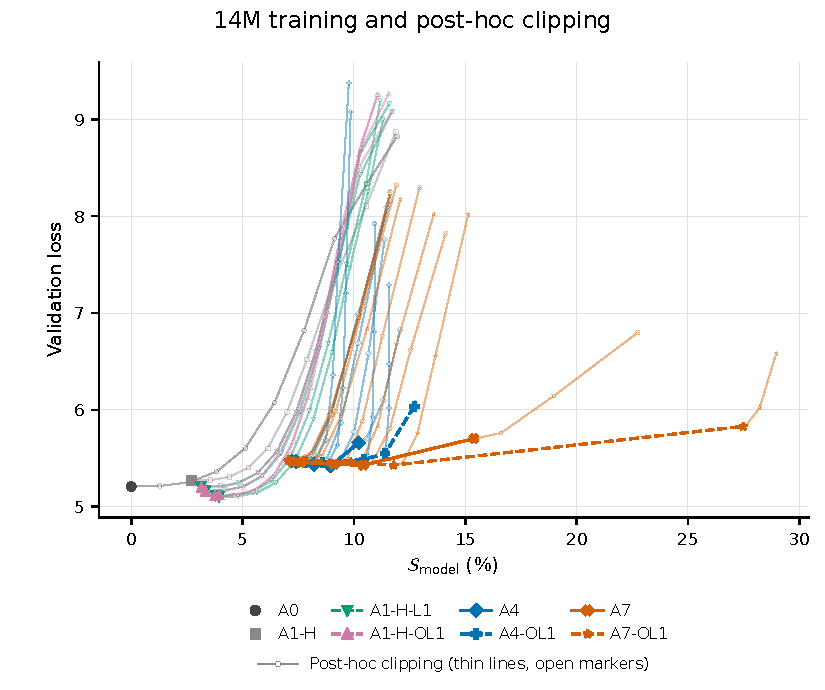
\includegraphics[width=\linewidth]{figures/appendix/14m-posthoc-frontiers.pdf}
\caption{Complete 14M training and post-hoc thresholding results: 30 trained
endpoints and 300 post-hoc thresholding evaluations. Large filled markers denote trained
endpoints; bold lines connect their settings, solid for unpressured recipes
and dashed for L1/OL1. Each faint open-marker path follows one fixed
checkpoint through $p=0,0.1,\ldots,0.9$. Colors and symbols identify its
source recipe. The full loss range is shown. Connections order evaluated
settings and do not interpolate attainable models or fitted Pareto envelopes.}
\label{fig:clipping-14m}
\end{figure}

\begin{figure}[htbp]
\centering
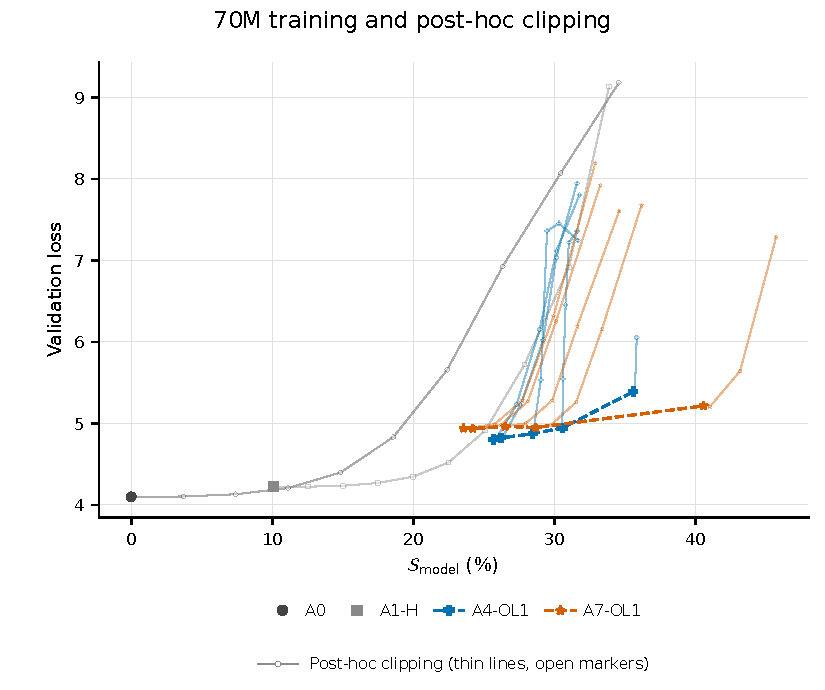
\includegraphics[width=\linewidth]{figures/appendix/70m-posthoc-frontiers.pdf}
\caption{Complete 70M training and post-hoc thresholding results: 12 trained
endpoints and 120 post-hoc thresholding evaluations. Large filled markers and bold
lines identify the trained recipes; faint open-marker paths follow each
checkpoint through ten increasing thresholding targets. All points, including
overlaps and high-loss settings, are retained. The evaluation and line
conventions match Figure~\ref{fig:clipping-14m}.}
\label{fig:clipping-70m}
\end{figure}

\FloatBarrier
\paragraph{410M as a fixed-token stress test.}
% Source: Analysis024 observations/031-quality-main-appendix.md;
% generating analysis: 23_plot_quality_main_appendix.py; original evidence: 20_plot_quality_all_sizes.py.
Figure~\ref{fig:quality-sparsity-410m} retains all twelve trained 410M
conditions and both complete control-clipping paths. At $\kappa=0.5$,
$T_7/P_{\mathrm{all}}$ reaches $80.62\%$ model-wide sparsity, or $92.4\%$
of the seven-site ceiling, at loss $5.121$ versus the base model's $4.547$.
This tests attainable sparsity under a larger architecture and the same token
budget; it is not a quality-scaling experiment. The 410M seven-site ceiling
is $87.25\%$, compared with $49.42\%$ at 70M, so greater architectural reach
also contributes to the larger observed model-wide sparsity.

The 410M base-model loss exceeds 70M's $4.100$. All sizes receive 712 optimizer
steps and 1.493B input tokens, corresponding to $106.14$, $21.20$ and $3.68$
tokens per parameter at 14M, 70M and 410M. The 410M schedule also has a lower
peak learning rate ($3\times10^{-4}$ rather than $10^{-3}$). These differences
may contribute to the non-monotonic quality ordering, but their effects are
not isolated. The training trajectories are retained in
Figure~\ref{fig:a0-optimization}. We therefore treat 410M as a limited
stress test and use 14M/70M for detailed intervention and runtime analysis.

\begin{figure}[!htbp]
\centering
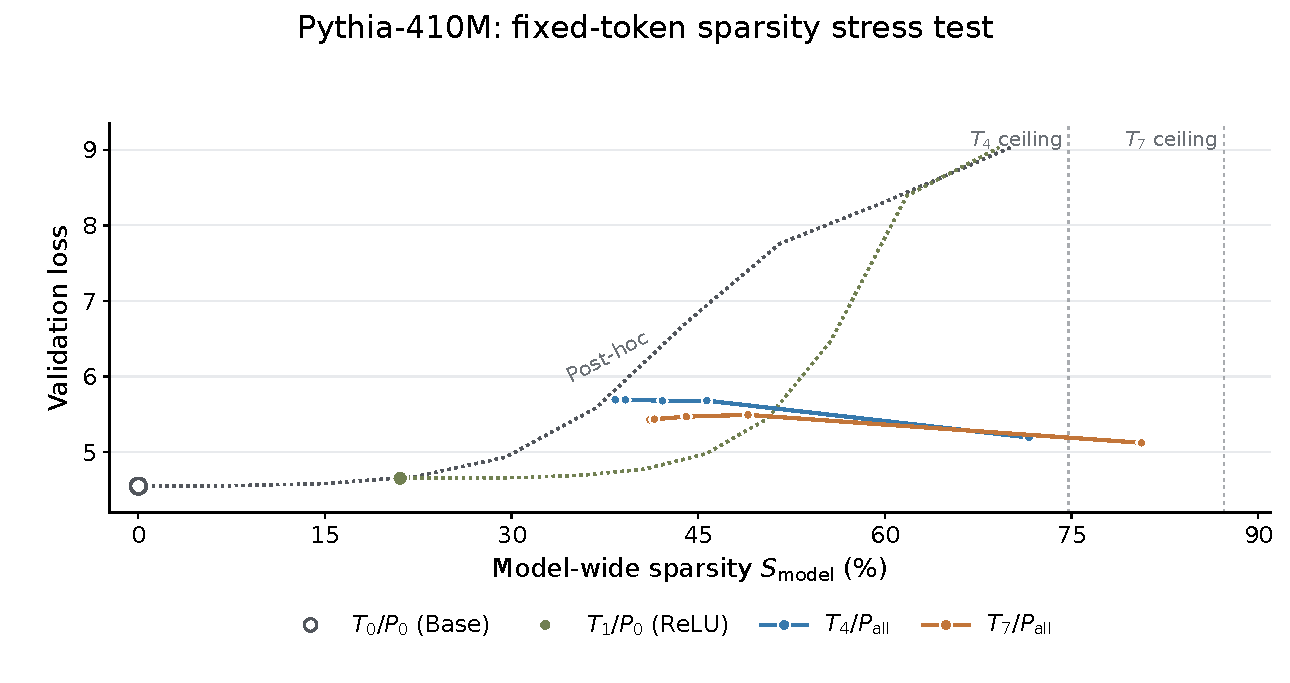
\includegraphics[width=\linewidth]{figures/appendix/A5-410m-quality-sparsity.pdf}
\caption{\textbf{Complete 410M quality--sparsity stress-test panel.}
All twelve trained conditions: Base, ReLU, and $T_4/P_{\mathrm{all}}$ and
$T_7/P_{\mathrm{all}}$ at $\kappa=0,.01,.05,.1,.5$. Dotted paths retain
all ten post-hoc targets for each fixed Base/ReLU control, including their
full loss range. Vertical guides mark the four- and seven-site sparsity
ceilings. Trained losses use ordinary final-checkpoint validation;
clipping retains its original FP16 pass. Sparsity pools logical counts over
all 338 complete validation blocks. Figure~\ref{fig:clipping-410m} additionally
retains the historical clipping sweeps of every trained recipe.}
\label{fig:quality-sparsity-410m}
\end{figure}

\begin{figure}[htbp]
\centering
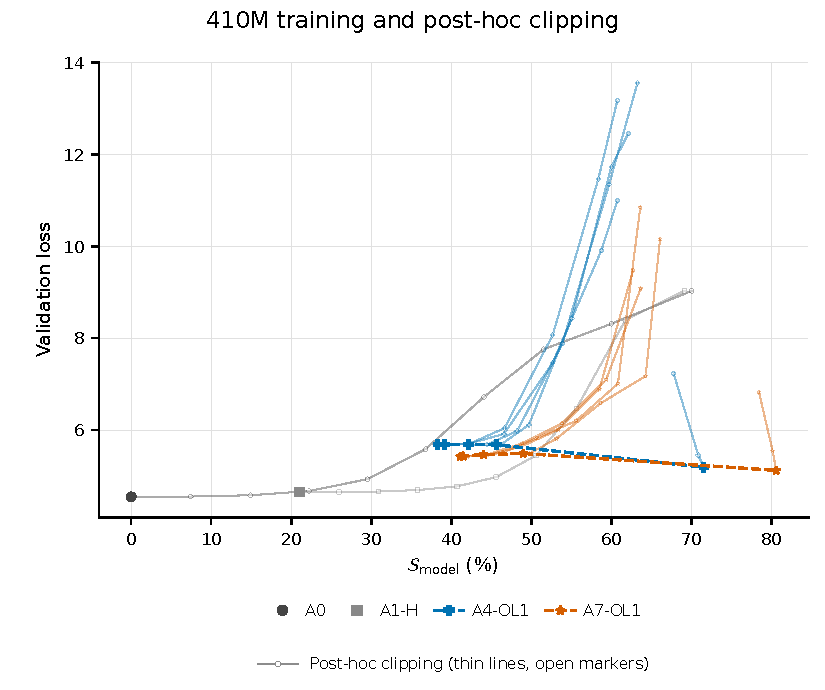
\includegraphics[width=\linewidth]{figures/appendix/410m-posthoc-frontiers.pdf}
\caption{Complete 410M training and post-hoc thresholding results: 12 trained
endpoints and 120 post-hoc thresholding evaluations. Large filled markers and bold
lines identify the trained recipes; faint open-marker paths follow each
checkpoint through ten increasing thresholding targets. All points, including
overlaps and high-loss settings, are retained. The evaluation and line
conventions match Figure~\ref{fig:clipping-14m}.}
\label{fig:clipping-410m}
\end{figure}

\FloatBarrier
% Consolidated implementation and evidence: Analysis024 Observation041.
% Evidence and audit: analyses/024-2026-09-17-h-only-kernel-latency/observations/041-kernel-appendix.md.
% Figure/data: Analysis024/31_kernel_appendix.py; data/kernel-appendix.json.
% Implementation: Run028 candidates/k050, k049, k042, k035; Run035 kernel/.
% Controlled tests: Run037 results/conditional-effects-audit.json; Run039 results/mechanism.json.
\subsection{Kernel development and evaluation}
\label{app:kernel-results}
\label{app:kernel-diagnostics}

\paragraph{Implementation.}
The specialized forward pass preserves each trained model's weights,
thresholds, biases and residual connections. It combines CUDA, CUTLASS and
FlashAttention components to fuse operations and skip matrix instructions
whose activation operands are zero. It introduces no additional pruning.
One kernel computes the two input LayerNorms from their shared input while
retaining separate affine parameters and thresholding. QKV layout conversion,
RoPE and the selected $q,k,v$ gates are fused; $q,k$ gates follow RoPE.
The FFN-down and attention-output projections are evaluated jointly with
their biases and residual addition. The final vocabulary projection remains
dense. Table~\ref{tab:kernel-paths} specifies the sparse execution rules.

\begin{table}[!htb]
\centering\small
\caption{\textbf{Sparse execution rules.} Tile dimensions are tokens by input
features. A matrix multiply--accumulate (MMA) instruction operates on
$16\times8\times16$ elements (output rows, output columns, reduction dimension).
Zero checks and any scalar replacement execute during every forward pass.}
\label{tab:kernel-paths}
\begin{tabularx}{\linewidth}{@{}p{.22\linewidth}XX@{}}
\toprule
Operation & Execution rule & Work avoided \\
\midrule
QKV, FFN-up ($a,m$) & Test each $16\times16$ activation fragment after both
operands have been loaded. & Skip the MMA for an empty fragment; retain operand reads. \\
FFN-down, attention output ($h,z$) & Inspect eight rows; use scalar arithmetic
for rows with at most two nonzeros when numerical guards pass. Process the
remaining rows in $8\times16$ tiles padded to 16 rows. & Skip empty tiles
before loading their weights. Scalar rows read only the corresponding weights. \\
Attention ($QK,PV$) & After loading the operands, use a warp-wide check to
test whether either complete MMA fragment is zero. & Skip that MMA; retain
input loading, masking, softmax and output processing. \\
\bottomrule
\end{tabularx}
\end{table}

The scalar path requires finite weights and biases, with nonzero magnitudes
between $2^{-50}$ and $2^{50}$; selected activations obey the same magnitude
bounds. Other rows use the matrix path. The two sizes retain these rules,
with projection dimensions adapted from $(d,d_f)=(128,512)$ to $(512,2048)$.
The 14M attention kernel uses $64\times256$ query/key tiles and two key/value
partitions; 70M uses $128\times128$ tiles without partitioning to match its
native attention reduction order. This change was needed for numerical
agreement, rather than selected by a 70M performance search.

\paragraph{Scope and numerical checks.}
Tests use one RTX\,5090, BF16 inference, batch size one, 2,048-token causal
sequences, and all 50,304 output logits, with PyTorch 2.11.0, Transformers
5.12.1 and CUDA 12.8. The implementation assumes fixed weights, shapes and
non-overlapping use of its buffers. It is not evaluated for training, cached
decoding, concurrent serving, arbitrary masks or thresholds outside the tested
grid. Each final checkpoint must pass in three fresh processes on all 338
validation sequences. Relative to the unmodified eager implementation, outputs
must be finite, every logit must satisfy
$|y-\hat y|\leq0.25+0.02|\hat y|$, the relative $\ell_2$ error of each sequence's
logits must not exceed $0.02$, and the absolute mean validation-loss difference
must not exceed $0.001$. These are numerical tolerances, not bitwise equivalence.

\paragraph{Timing and reference.}
Native PyTorch/SDPA and specialized inference use CUDA graphs with identical
inputs. Latency is the geometric mean of host timings over 64 fixed validation
sequences, seven randomized paired passes and three fresh processes.
Compilation, static weight layout preparation, graph capture and equal input
staging are excluded. Embeddings, all blocks, final normalization, vocabulary
logits and input-dependent preprocessing are included. Post-hoc masks also
remain inside timing; no activations are cached. Measurements use separate
GPU sessions, so common normalization does not remove session effects.

For comparisons across recipes, Figure~\ref{fig:kernel-diagnostics} uses
\emph{one native base-model latency per size}:
$t_{\mathrm{native},T_0/P_0}/t_{\mathrm{specialized},r}$ for recipe $r$.
The native references are 0.65544\,ms at 14M and 1.66388\,ms at 70M.
This differs from Figure~\ref{fig:base-model-speedup}, which uses the
specialized base-model latencies, 0.65157 and 3.31325\,ms.
The best trained-recipe gains are therefore $1.427\times$ and $1.028\times$
over the native base, versus $1.418\times$ and $2.047\times$ over the
specialized base. The latter 70M ratio reflects a slow dense path in the
ported implementation and does not establish a twofold gain over native inference.

\paragraph{What MMA bypass measures.}
Bypass is the number of omitted MMA instructions divided by issued plus
omitted instructions, pooling integer counts across layers and validation
sequences. Projection totals pool the four projection operations; attention
totals pool $QK$ and $PV$. We keep the two groups separate because equal
instruction counts need not imply equal costs. At $h,z$, bypass includes
replacement by scalar arithmetic and counts padded rows; it is not a fraction
of all arithmetic eliminated. Attention counts include causal padding:
even the base model bypasses $10.42\%$ of $PV$ instructions at 14M and
$5.15\%$ at 70M. In contrast, $\Smodel$ excludes masked pairs and includes
the dense vocabulary projection in its denominator.

The figure's projection scalar sparsity pools zero-activation products over
all projection products in the actual BF16 operands. Both this measure and
bypass cover all 338 validation sequences; timing uses the 64-sequence subset.
Thus these diagnostics complement, rather than redefine, the canonical
model-wide sparsity used in the quality figures.

\begin{figure}[!htb]
\centering
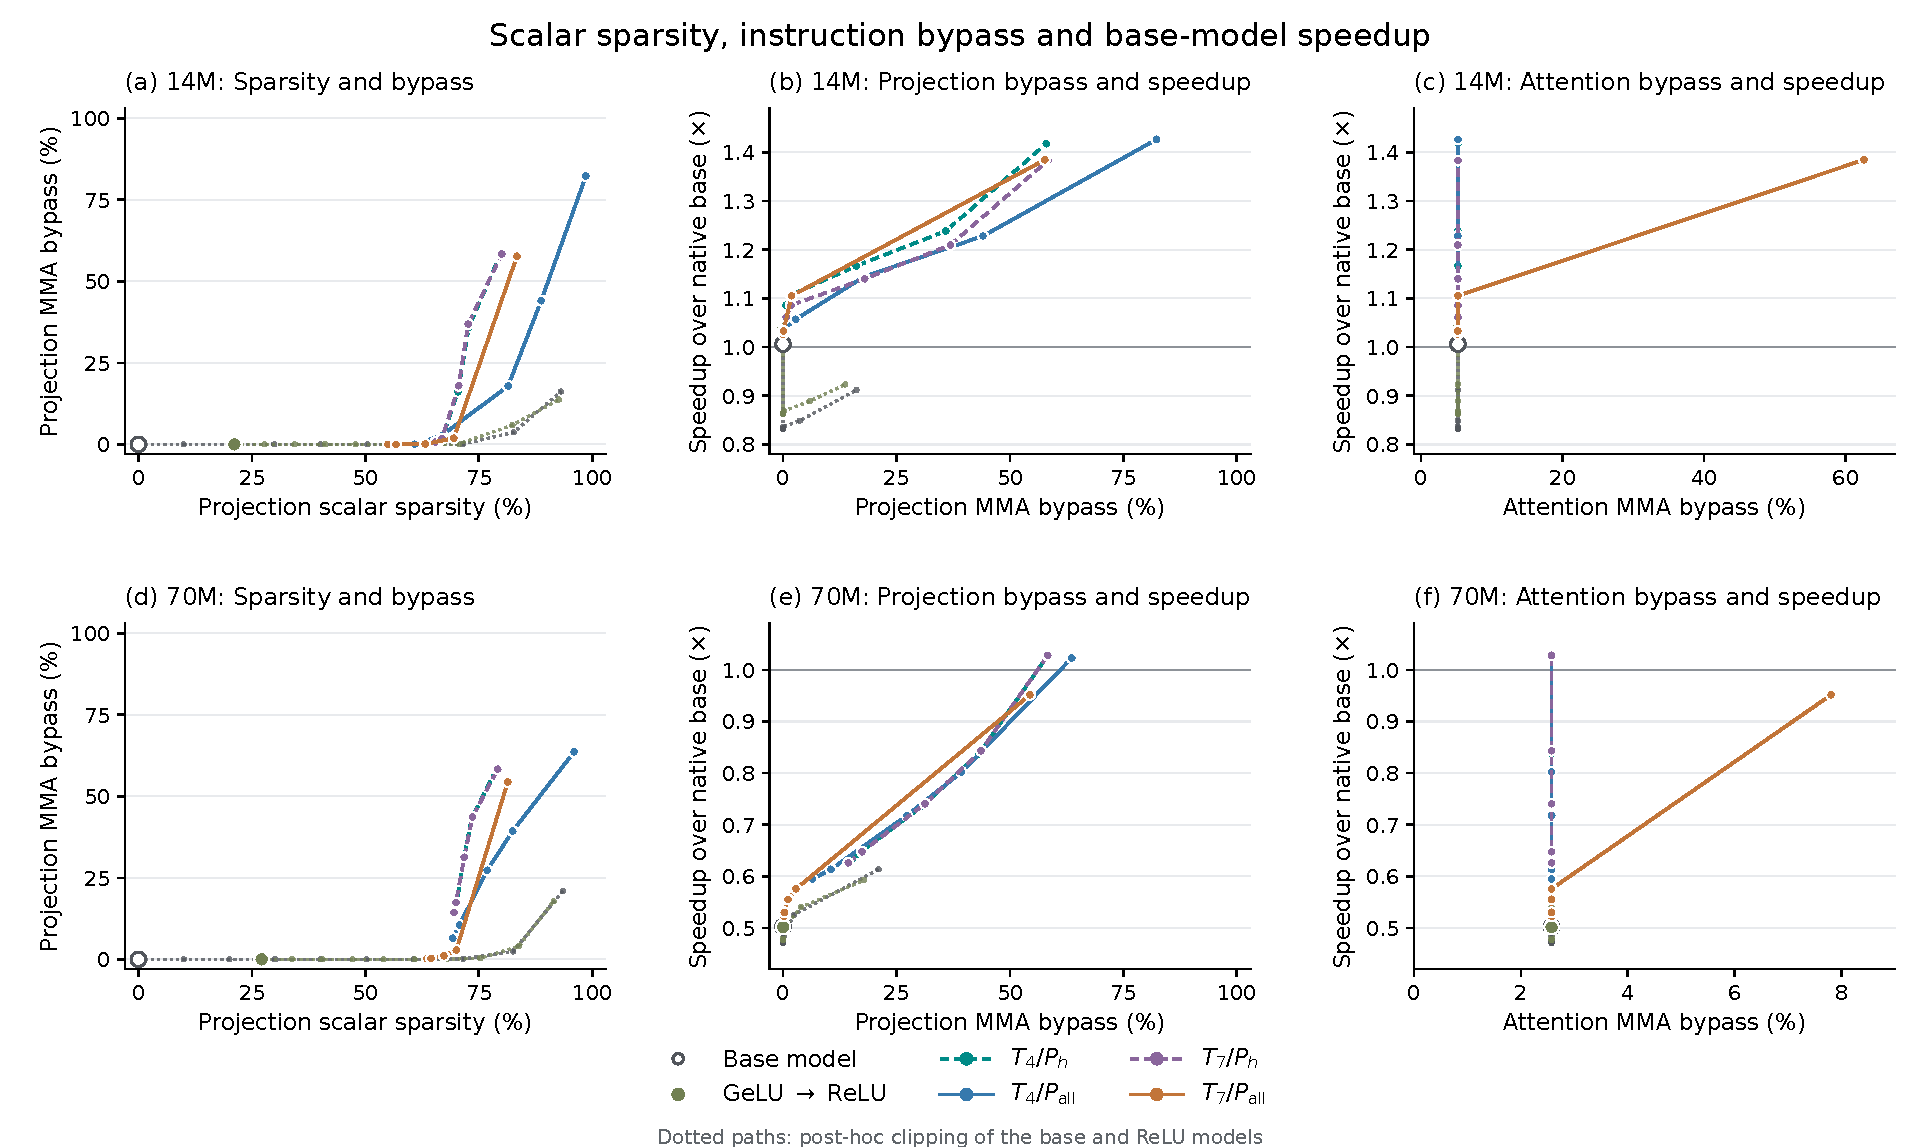
\includegraphics[width=\linewidth]{figures/20-kernel-structure-native-base-speedup.pdf}
\caption{\textbf{Scalar sparsity, instruction bypass and speedup over a fixed
native base model.} Rows show 14M and 70M, each with 22 trained settings and
20 post-hoc control settings. Left: projection scalar sparsity versus projection
MMA bypass. Middle/right: projection/attention bypass versus full-model speedup.
Every speedup within a row uses the same native $T_0/P_0$ reference; the
horizontal line is $1\times$. The Base model marker uses specialized inference,
so it need not lie on that line. Lines connect measured thresholds, not fitted
trends; dotted paths are post-hoc clipping. Counts are pooled, include the
instruction-padding and scalar-substitution conventions above, and do not
measure saved memory traffic.}
\label{fig:kernel-diagnostics}
\end{figure}

\paragraph{Interpretation and controlled tests.}
Projection bypass tracks speedup in both sizes, but high scalar sparsity alone
need not produce empty instruction tiles. Post-hoc controls show this gap and
incur separate masking costs. Attention bypass is nearly constant across the
trained grid except for $T_7/P_{\mathrm{all}}$ at $\kappa=0.5$; this single
exception cannot establish a general attention-speedup relation. At 70M it
has more attention bypass but less native-base speedup than $T_7/P_h$
($0.952\times$ versus $1.028\times$). Bypass therefore describes exploitable
structure without explaining all latency differences.

Table~\ref{tab:kernel-mechanisms} provides the direct 14M test: disable one
skipping path while keeping weights, gates and fusion fixed. Its min--max
spans cover all pairs of three independent off/on process means; effects are
conditional and non-additive. These tests do not separately time memory reads,
zero checks or softmax. No corresponding operation-level ablation was run at
70M, so its scatter is descriptive evidence, not causal attribution.

\paragraph{Alternatives tested.}
Porting the $h,z$ strategy to $a,m$ was correct but slower in the tested 14M
case (Section~\ref{sec:kernel-autoresearch}). The padded fallback issued
$1.90\times$ and $2.00\times$ as many matrix instructions, respectively.
Attention shortcuts using cumulative value sums for zero queries, disjoint
query/key supports, or cheaper conditional execution either failed numerical
checks or did not establish a reliable gain. Disabling attention skipping
improved all 35 historical 14M comparisons. The retained implementation is
therefore not latency-optimal; it preserves one common execution policy across
recipes. Earlier detection that avoids attention operand reads, fused post-hoc
masking and sparsification of softmax probabilities remain untested here.


